
\chapter{Fundamental Group}

Motivation. The fundamental group connects topology and algebra together, by labelling a group to each topological space, which is known as fundamental group.

Why do we need algebra in topology. Consider the \({S}^{2}\) (2-shpere) and \({S}^{1} \times  {S}^{1}\)

(torus):

\begin{center}
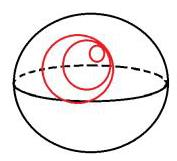
\includegraphics[max width=0.2\textwidth]{images/bo_d2bcsrref24c73avs720_112_711_510_177_161_0.jpg}
\end{center}
\hspace*{3em} 

Figure 11.8: Any loop in the sphere can be contracted into a point

\begin{center}
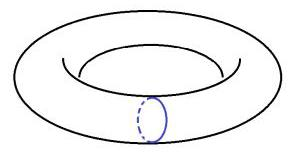
\includegraphics[max width=0.2\textwidth]{images/bo_d2bcsrref24c73avs720_112_656_964_289_152_0.jpg}
\end{center}
\hspace*{3em} 

Figure 11.9: Some loops in the torus cannot be contracted into a point

As can be seen from Fig.(11.8) and Fig.(11.9), any "loop" on a sphere can be contracted to a point, while some "loop" on a torus cannot. We need the algebra to describe this phenomena formally.

Definition 11.7 [loop] Let \(X\) be a topological space. A loop on \(X\) is a constant map \(\ell  : \left\lbrack  {0,1}\right\rbrack   \rightarrow  X\) such that \(\ell \left( 0\right)  = \ell \left( 1\right)\) .

We say \(\ell\) is based at \(b \in  X\) if \(\ell \left( 0\right)  = \ell \left( 1\right)  = b\) .

Definition 11.8 [composite loop] Suppose that \(\mathbf{u},\mathbf{v}\) are loops on \(X\) based at \(b \in  X\) . The composite loop \(u \cdot  v\) is given by

\[
u \cdot  v = \left\{  \begin{array}{rr} u\left( {2t}\right) , & \text{ if }0 \leq  t \leq  1/2 \\  v\left( {{2t} - 1}\right) , & \text{ if }1/2 \leq  t \leq  1 \end{array}\right.
\]

Definition 11.9 [fundamental group] The homotopy class of loops relative to \(\{ 0,1\}\) based at \(b \in  X\) forms a group. It is called the fundamental group of \(X\) based at \(b\) , denoted as \({\pi }_{1}\left( {X,b}\right)\) .

More precisely, let

\(\left\lbrack  \ell \right\rbrack   = \{ m \mid  m\) is a loop based at \(b\) that is homotopic to \(\ell\) , relative to \(\{ 0,1\} \}\) ,

and \({\pi }_{1}\left( {X,b}\right)  = \{ \left\lbrack  \ell \right\rbrack   \mid  \ell\) are loops based at \(b\}\) . The operation in \({\pi }_{1}\left( {X,b}\right)\) is defined as:

\[
\left\lbrack  \ell \right\rbrack   * \left\lbrack  {\ell }^{\prime }\right\rbrack   \mathrel{\text{ := }} \left\lbrack  {\ell  \cdot  {\ell }^{\prime }}\right\rbrack  ,\;\forall \left\lbrack  \ell \right\rbrack  ,\left\lbrack  {\ell }^{\prime }\right\rbrack   \in  {\pi }_{1}\left( {X,b}\right) .
\]

R Two paths \({\ell }_{1},{\ell }_{2} : \left\lbrack  {0,1}\right\rbrack   \rightarrow  X\) are homotopic relative to \(\{ 0,1\}\) if we can find \(H : \left\lbrack  {0,1}\right\rbrack   \times  \left\lbrack  {0,1}\right\rbrack   \rightarrow  X\) such that

\[
H\left( {t,0}\right)  = {\ell }_{1}\left( t\right) ,\;H\left( {t,1}\right)  = {\ell }_{2}\left( t\right)
\]

and

\[
H\left( {0,s}\right)  = {\ell }_{1}\left( 0\right)  = {\ell }_{2}\left( 0\right) ,\forall 0 \leq  s \leq  1,\;H\left( {1,s}\right)  = {\ell }_{1}\left( 1\right)  = {\ell }_{2}\left( 1\right) ,\forall 0 \leq  s \leq  1
\]

Counter example for homotopy but not relative to \(\{ 0,1\}\) :

\begin{center}
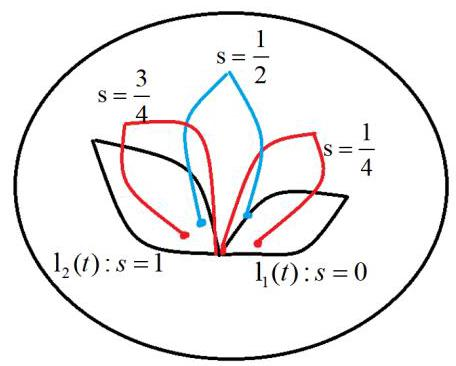
\includegraphics[max width=0.3\textwidth]{images/bo_d2bcsrref24c73avs720_113_744_1658_456_366_0.jpg}
\end{center}
\hspace*{3em} 

Figure 11.10: homotopy not relative to \(\{ 0,1\}\)

\section*{11.6. Wednesday for MAT4002}

\section*{11.6.1.The fundamental group}

Revewing. One example for Homotopy relative to \(\{ 0,1\}\) is illustrated in Fig.(11.4)

\begin{center}
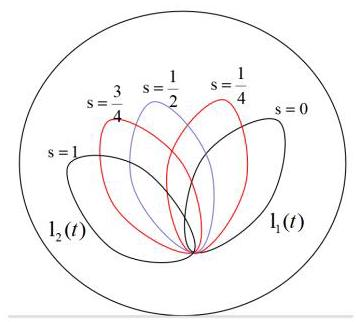
\includegraphics[max width=0.3\textwidth]{images/bo_d2bcsrref24c73avs720_114_646_571_356_322_0.jpg}
\end{center}
\hspace*{3em} 

Figure 11.11: Example of homotopy relative to \(\{ 0,1\}\)

It’s essential to study homotopy relative to \(\{ 0,1\}\) . For example, given a torus with a loop \({\ell }_{1}\left( t\right)\) and a base point \(b\) . We want to distinguish \({\ell }_{1}\left( t\right)\) and \({\ell }_{2}\left( t\right)\) as shown in Fig.(11.12):

\begin{center}
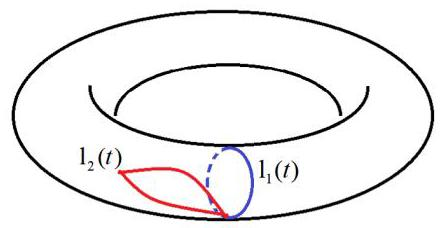
\includegraphics[max width=0.3\textwidth]{images/bo_d2bcsrref24c73avs720_114_596_1228_442_228_0.jpg}
\end{center}
\hspace*{3em} 

Figure 11.12: Two loops on a torus

Obviously there should be something different between \({\ell }_{1}\left( t\right)\) and \({\ell }_{2}\left( t\right)\) . "Relative to \(\{ 0,1\}\) is essential", sicne if we get rid of this condition, all loops are homotopic to the constant map \({c}_{b}\left( t\right)  = b\) . See the graphic illustration in Fig.(??):

\begin{center}
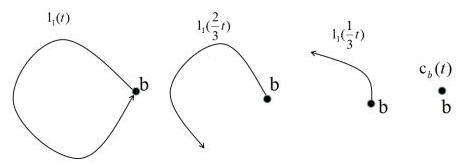
\includegraphics[max width=0.3\textwidth]{images/bo_d2bcsrref24c73avs720_114_591_1782_464_166_0.jpg}
\end{center}
\hspace*{3em} 

Figure 11.13: homotopy between any loop and constant map

In this case, \(\ell  \simeq  {c}_{b}\) for any loop \(\ell\) , there is only one trivial element \(\left\{  \left\lbrack  {c}_{b}\right\rbrack  \right\}\) in \({\pi }_{1}\left( {X,b}\right)\) .

That’s the reason why we define \({\pi }_{1}\left( {X,b}\right)\) as the collection of homotopy classes relative to \(\{ 0,1\}\) based at \(b\) in \(X\) .

Proposition 11.13 Let \(\left\lbrack  \cdot \right\rbrack\) denote the homotopy class of loops relative to \(\{ 0,1\}\) based at \(b\) , and define the operation

\[
\left\lbrack  \ell \right\rbrack   * \left\lbrack  {\ell }^{\prime }\right\rbrack   = \left\lbrack  {\ell  \cdot  {\ell }^{\prime }}\right\rbrack
\]

Then \(\left( {{\pi }_{1}\left( {X,b}\right) , * }\right)\) forms a group, where

\[
{\pi }_{1}\left( {X,b}\right)  \mathrel{\text{ := }} \{ \left\lbrack  \ell \right\rbrack   \mid  \ell  : \left\lbrack  {0,1}\right\rbrack   \rightarrow  X\text{ denotes loops based at }b\}
\]

Proof. 1. Well-definedness: Suppose that \(u \sim  {u}^{\prime }\) and \(v \sim  {v}^{\prime }\) , it suffices to show \(u \cdot  v \simeq\)  \({u}^{\prime } \cdot  {v}^{\prime }\) . Consider the given homotopies \(H : u \simeq  {u}^{\prime },K : v \simeq  {v}^{\prime }\) . Construct a new homotopy \(L : I \times  I \rightarrow  X\) by

\[
L\left( {t,s}\right)  = \left\{  \begin{array}{rr} H\left( {{2t},s}\right) , & 0 \leq  t \leq  1/2 \\  K\left( {{2t} - 1,s}\right) , & 1/2 \leq  t \leq  1 \end{array}\right.
\]

The diagram below explains the ideas for constructing \(L\) . The plane denote the set \(I \times  I\) , and the labels characterize the images of each point of \(I \times  I\) under \(L\) . Therefore, \(u \cdot  v \simeq  {u}^{\prime } \cdot  {v}^{\prime }\) .

\begin{center}
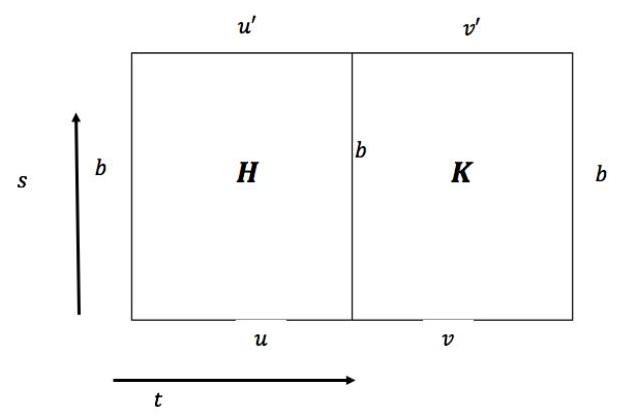
\includegraphics[max width=0.5\textwidth]{images/bo_d2bcsrref24c73avs720_115_639_1586_617_417_0.jpg}
\end{center}
\hspace*{3em} 

2. Associate: \(\left( {u \cdot  v}\right)  \cdot  w \simeq  u \cdot  \left( {v \cdot  w}\right)\)

Note that \(\left( {u \cdot  v}\right)  \cdot  w\) and \(u \cdot  \left( {v \cdot  w}\right)\) are essentially different loops. Although they go with the same path, they are with different speeds. Generally speaking, the loop \(\left( {u \cdot  v}\right)  \cdot  w\) travels \(u,v\) using \(1/4\) seconds, and \(w\) in \(1/2\) seconds; but the loop \(u \cdot  \left( {v \cdot  w}\right)\) travels \(u\) in \(1/2\) seconds, and then \(v,w\) in \(1/4\) seconds.

We want to construct a homotopy that describes the loop changes from \(u \cdot  \left( {v \cdot  w}\right)\) to \(\left( {u \cdot  v}\right)  \cdot  w\) . A graphic illustration is given below:

\begin{center}
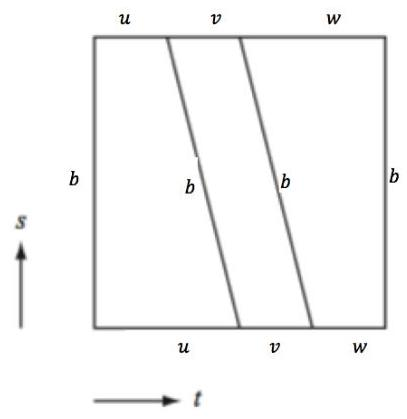
\includegraphics[max width=0.3\textwidth]{images/bo_d2bcsrref24c73avs720_116_621_761_407_419_0.jpg}
\end{center}
\hspace*{3em} 

An explicit homotopy \(H : I \times  I \rightarrow  X\) is given below:

\[
H\left( {t,s}\right)  = \left\{  \begin{matrix} u\left( {{4t}/\left( {2 - s}\right) }\right) , & 0 \leq  t \leq  1/2 - 1/{4s} \\  v\left( {{4t} - 2 + s}\right) , & 1/2 - 1/{4s} \leq  t \leq  3/4 - 1/{4s} \\  w\left( {{4t} - 3 + s/\left( {1 + s}\right) }\right) , & 3/4 - 1/{4s} \leq  t \leq  1 \end{matrix}\right.
\]

Therefore,

\[
\left\lbrack  u\right\rbrack   * \left( {\left\lbrack  v\right\rbrack   * \left\lbrack  w\right\rbrack  }\right)  = \left( {\left\lbrack  u\right\rbrack   * \left\lbrack  v\right\rbrack  }\right)  * \left\lbrack  w\right\rbrack
\]

3. Intuitively, the identity should be the constant map, i.e., let \({c}_{b} : I \rightarrow  X\) by \({c}_{b}\left( t\right)  =\)

\(b,\forall t\) , and let \(\ell  = \left\lbrack  {c}_{b}\right\rbrack\) , it suffices to show

\[
\left\lbrack  {c}_{b}\right\rbrack   * \left\lbrack  \ell \right\rbrack   = \left\lbrack  \ell \right\rbrack   * \left\lbrack  {c}_{b}\right\rbrack   = \left\lbrack  \ell \right\rbrack   \Leftrightarrow  \left\lbrack  {{c}_{b} \cdot  \ell }\right\rbrack   = \left\lbrack  {\ell  \cdot  {c}_{b}}\right\rbrack   = \left\lbrack  \ell \right\rbrack
\]

Or equivalently,

\[
{c}_{b} \cdot  \ell  \simeq  \ell ,\;\ell  \cdot  {c}_{b} \simeq  \ell
\]

The graphic homotopy is shown below. (You should have been understood this diagram)

\begin{center}
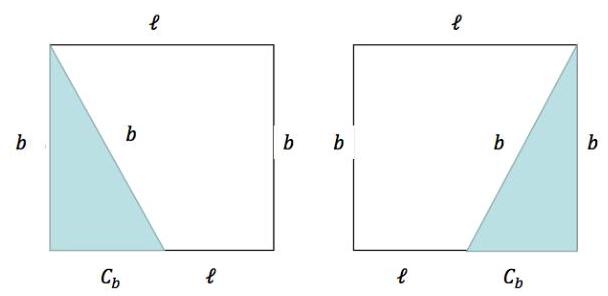
\includegraphics[max width=0.5\textwidth]{images/bo_d2bcsrref24c73avs720_117_655_468_608_296_0.jpg}
\end{center}
\hspace*{3em} 

4. Inverse: the inverse of \(\left\lbrack  u\right\rbrack\) , where \(u\) is a loop, should be \(\left\lbrack  {u}^{\prime }\right\rbrack\) , where \({u}^{\prime }\) is the reverse of the traveling of \(u\) . Therefore, for all \(u : I \rightarrow  X\) (loop based at \(b\) ), define \({u}^{-1} : I \rightarrow  X\) by \({u}^{-1}\left( t\right)  = u\left( {1 - t}\right)\) . Note that

\[
\left\lbrack  u\right\rbrack   * \left\lbrack  {u}^{-1}\right\rbrack   = \left\lbrack  {u \cdot  {u}^{-1}}\right\rbrack  ,\;e = \left\lbrack  {c}_{b}\right\rbrack
\]

It suffices to show \(u \cdot  {u}^{-1} \simeq  {c}_{b}\) and \({u}^{-1} \cdot  u \simeq  {c}_{b}\) :

The homotopy below gives \(u \cdot  {u}^{-1} \simeq  {c}_{b}\) , and the \({u}^{-1} \cdot  u \simeq  {c}_{b}\) follows similarly.

\[
H\left( {t,s}\right)  = \left\{  \begin{array}{rr} u\left( {{2t}\left( {1 - s}\right) }\right) , & 0 \leq  t \leq  1/2 \\  u\left( {\left( {2 - {2t}}\right) \left( {1 - s}\right) }\right) , & 1/2 \leq  t \leq  1 \end{array}\right.
\]

The graphic illustration is given below:

\begin{center}
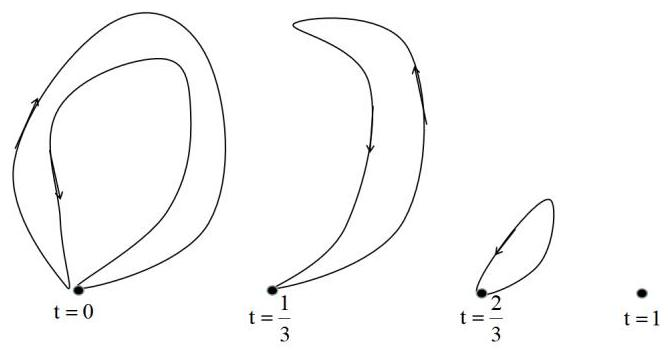
\includegraphics[max width=0.5\textwidth]{images/bo_d2bcsrref24c73avs720_117_636_1629_668_351_0.jpg}
\end{center}
\hspace*{3em} 

Note that the figure below does not define a homotopy from \(u \cdot  {u}^{-1}\) to \({c}_{b}\) !

\begin{center}
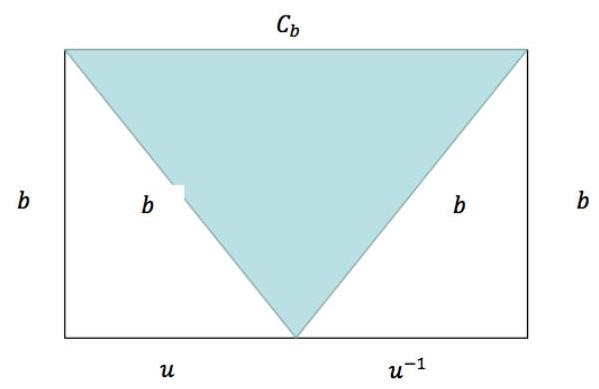
\includegraphics[max width=0.5\textwidth]{images/bo_d2bcsrref24c73avs720_118_529_423_599_389_0.jpg}
\end{center}
\hspace*{3em} 

The reason is that for the upper part, as \(s \rightarrow  1\) , the time for traveling \(u\) and \({u}^{-1}\) becomes very small, i.e., a particle has to pass \(u\) and \({u}^{-1}\) in infinitely small time, which is not well-defined.

\begin{itemize}
\item Example 11.11 The reason why \({\pi }_{1}\left( {{\mathbb{R}}^{2},b}\right)  = \{ e\}\) is trivial:
\end{itemize}

\begin{itemize}
\item For any \(u : I \rightarrow  {\mathbb{R}}^{2}\) with \(u\left( 0\right)  = u\left( 1\right)  = b\) , consider the homotopy
\end{itemize}

\[
H\left( {t,s}\right)  = \left( {1 - s}\right) u\left( t\right)  + {sb}.
\]

Therefore, \(u \simeq  {c}_{b}\) for any loop \(u\) based at \(b\) . Check the diagram below for graphic illustration of this homotopy.

\begin{center}
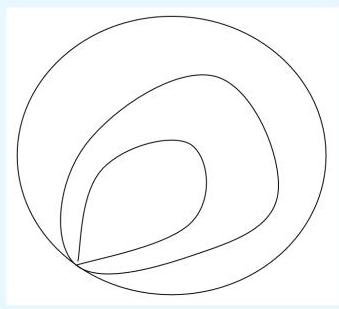
\includegraphics[max width=0.2\textwidth]{images/bo_d2bcsrref24c73avs720_118_659_1622_339_309_0.jpg}
\end{center}
\hspace*{3em} 

More generally, if \(X \simeq  \{ x\}\) is contractible, then \({\pi }_{1}\left( {X,b}\right)  = \{ e\}\) . The same argument cannot work for \(\left( {{\mathbb{R}}^{2}\{ 0\} ,\mathbf{b}}\right)\) , since the mapping \(H : {\mathbb{R}}^{2} \smallsetminus  \{ 0\}  \times  I \rightarrow  {\mathbb{R}}^{2} \smallsetminus  \{ 0\}\) with

\(H\left( {\mathbf{t},s}\right)  = \left( {1 - s}\right) u\left( \mathbf{t}\right)  + s\mathbf{b}\) is not well-defined. In particular, the value \(H\left( {s,t}\right)\) may hit the origin0.

However, \({\pi }_{1}\left( {{S}^{1},1}\right)\) is non-trivial. We cannot deform the loop in \({S}^{1}\) into a constant loop. We will see that \({\pi }_{1}\left( {{S}^{1},1}\right)  \cong  \mathbb{Z}\) .

Proposition 11.14 If \(b,{b}^{\prime }\) are path-connected in \(X\) , then \({\pi }_{1}\left( {X,b}\right)  \cong  {\pi }_{1}\left( {X,{b}^{\prime }}\right)\) .

Proof. Let \(w\) be a path from \(b\) to \({b}^{\prime }\) , and define

\[
{w}_{\# } : \;{\pi }_{1}\left( {X,b}\right)  \rightarrow  {\pi }_{1}\left( {X,{b}^{\prime }}\right)
\]

\[
\text{ with }\left\lbrack  \ell \right\rbrack   \mapsto  \left\lbrack  {{w}^{-1}\ell w}\right\rbrack
\]

1. Well-definedness: Check that \(\ell  \simeq  {\ell }^{\prime }\) implies \({w}^{-1}\ell w \simeq  {w}^{-1}{\ell }^{\prime }w\) . See the figure below for graphic illustration.

\begin{center}
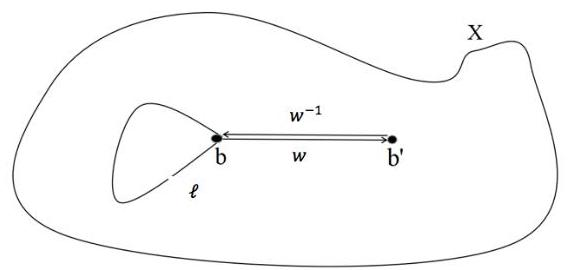
\includegraphics[max width=0.4\textwidth]{images/bo_d2bcsrref24c73avs720_119_683_1166_568_270_0.jpg}
\end{center}
\hspace*{3em} 

2. \({w}_{\# }\) is a homomorphism:

\[
{w}_{\# }\left( \left\lbrack  {\ell }_{1}\right\rbrack  \right)  \cdot  {w}_{\# }\left( \left\lbrack  {\ell }_{2}\right\rbrack  \right)  = \left\lbrack  {{w}^{-1} \cdot  {\ell }_{1}w}\right\rbrack   \cdot  \left\lbrack  {{w}^{-1} \cdot  {\ell }_{2}w}\right\rbrack   \tag{11.4a}
\]

\[
= \left\lbrack  {{w}^{-1} \cdot  {\ell }_{1}{\ell }_{2}w}\right\rbrack   \tag{11.4b}
\]

\[
= {w}_{\# }\left( \left\lbrack  {{\ell }_{1}{\ell }_{2}}\right\rbrack  \right)  \tag{11.4c}
\]

where (11.4b) is because that \(w \cdot  {w}^{-1} = {c}_{b}\) .

3. And \({w}_{\# }\) is also injective. If loops \({\ell }_{1},{\ell }_{2}\) are such that \({w}_{\# }\left( {\ell }_{1}\right)  = {w}_{\# }\left( {\ell }_{2}\right)\) , then

\[
\left\lbrack  {{w}^{-1}{\ell }_{1}w}\right\rbrack   = \left\lbrack  {{w}^{-1}{\ell }_{2}w}\right\rbrack
\]

which follows that

\[
\left\lbrack  {\ell }_{1}\right\rbrack   = \left\lbrack  w\right\rbrack  \left\lbrack  {{w}^{-1}{\ell }_{1}w}\right\rbrack  \left\lbrack  {w}^{-1}\right\rbrack   = \left\lbrack  w\right\rbrack  \left\lbrack  {{w}^{-1}{\ell }_{2}w}\right\rbrack  \left\lbrack  {w}^{-1}\right\rbrack   = \left\lbrack  {\ell }_{2}\right\rbrack   \tag{11.5}
\]

4. Finally, \({w}_{\# }\) is surjective, because for any \(u \in  {\pi }_{1}\left( {X,{b}^{\prime }}\right)\) , let \(v = {wu}{w}^{-1}\) , then \(v\) is based at \(b\) , so \(\left\lbrack  v\right\rbrack   \in  {\pi }_{1}\left( {X,b}\right)\) , and \({w}_{\# }\left( v\right)  = \left\lbrack  u\right\rbrack\) . Therefore \({w}_{\# }\) is surjective.

In conclusion, \({w}_{\# }\) is a group isomorphism between \({\pi }_{1}\left( {X,b}\right)\) and \({\pi }_{1}\left( {X,{b}^{\prime }}\right)\) .

In (11.5) we extended the meaning of \(\left\lbrack  \ell \right\rbrack\) to allow \(\ell\) to be a path, and the equivalence class is defined by the relation " \(\sim\) ": \({\ell }_{1} \sim  {\ell }_{2}\) iff they are homotopic relative to \(\{ 0,1\}\) . The multiplication rules are defined similarly.

\section*{12.3. Monday for MAT4002}

Proposition 12.3 If \(b,{b}^{\prime }\) are path connected in \(X\) , then

\[
{\pi }_{1}\left( {X,b}\right)  \cong  {\pi }_{1}\left( {X,{b}^{\prime }}\right)
\]

R Last lecture we have given the isomorphism

\[
{W}_{\# } : \;{\pi }_{1}\left( {X,b}\right)  \rightarrow  {\pi }_{1}\left( {X,{b}^{\prime }}\right)
\]

\[
\text{ with }\left\lbrack  \ell \right\rbrack   \mapsto  \left\lbrack  {{w}^{-1} \cdot  \ell  \cdot  w}\right\rbrack
\]

where \(w\) denotes a path from \(b\) to \({b}^{\prime }\) . The inverse of \({W}_{\# }\) is given by:

\[
{W}_{\# }^{-1} : \;{\pi }_{1}\left( {X,{b}^{\prime }}\right)  \rightarrow  {\pi }_{1}\left( {X,b}\right)
\]

\[
\text{ with }\left\lbrack  m\right\rbrack   \mapsto  \left\lbrack  {w \cdot  m \cdot  {w}^{-1}}\right\rbrack
\]

Notation. For path connected space \(X\) , we will just write \({\pi }_{1}\left( X\right)\) instead of \({\pi }_{1}\left( {X,x}\right)\) .

Proposition 12.4 Let(X, x)and(Y, y)be spaces with basepoints \(x\) and \(y\) , and \(f : X \rightarrow  Y\) be a continuous map with \(f\left( x\right)  = y\) . Then every loop \(\ell  : I \rightarrow  X\) based at \(x\) gives a loop \(f \circ  \ell  : I \rightarrow  Y\) based at \(y\) , i.e., the continous map \(f\) induces a homomorphism of groups

\[
{f}_{ * } : \;{\pi }_{1}\left( {\pi ,x}\right)  \rightarrow  {\pi }_{1}\left( {Y,y}\right)
\]

\[
\left\lbrack  \ell \right\rbrack   \mapsto  \left\lbrack  {f \circ  \ell }\right\rbrack   \mathrel{\text{ := }} {f}_{ * }\left( \left\lbrack  \ell \right\rbrack  \right)
\]

Moreover,

1. \({\left( {\operatorname{id}}_{X \rightarrow  X}\right) }_{ * } = {\operatorname{id}}_{{\pi }_{1}\left( {X,x}\right)  \rightarrow  {\pi }_{1}\left( {X,x}\right) }\)

2. \({\left( g \circ  f\right) }_{ * } = {g}_{ * } \circ  {f}_{ * }\)

3. If \(f \simeq  {f}^{\prime }\) relative to \(x \in  X\) , then \({f}_{ * } = {\left( {f}^{\prime }\right) }_{ * }\)

Proof. - Well-definedness: Suppose that \(\ell  \simeq  {\ell }^{\prime }\) , then \(f \circ  \ell  \simeq  f \circ  {\ell }^{\prime }\) by propositon (9.4).

Therefore, \(\left\lbrack  {f \circ  \ell }\right\rbrack   = \left\lbrack  {f \circ  {\ell }^{\prime }}\right\rbrack\) .

\begin{itemize}
\item Homomorphism: It's clear that
\end{itemize}

\[
f \circ  \left( {\ell  \circ  {\ell }^{\prime }}\right)  = \left( {f \circ  \ell }\right)  \circ  \left( {f \circ  {\ell }^{\prime }}\right)
\]

Therefore, \({f}_{ * }\left\lbrack  {\ell {\ell }^{\prime }}\right\rbrack   = \left( {{f}_{ * }\left\lbrack  \ell \right\rbrack  }\right)  * \left( {{f}_{ * }\left\lbrack  {\ell }^{\prime }\right\rbrack  }\right)\)

The other three statements are obvious.

Proposition 12.5 Let \(X,Y\) be path-connected such that \(X \simeq  Y\) (i.e., there exists \(f : X \rightarrow  Y\) and \(g : Y \rightarrow  X\) such that \(g \circ  f \simeq  {\operatorname{id}}_{X},f \circ  g \simeq  {\operatorname{id}}_{Y}\) ). Then \({\pi }_{1}\left( X\right)  \cong  {\pi }_{1}\left( Y\right)\) .

In particular, if \(X,Y\) are path-connected with \(X \cong  Y\) , then \({\pi }_{1}\left( X\right)  \cong  {\pi }_{1}\left( Y\right)\)

Proof. Consider the mapping

\[
{\pi }_{1}\left( {X,{x}_{0}}\right) \overset{{f}_{ * }}{ \rightarrow  }{\pi }_{1}\left( {Y,{y}_{0}}\right) \overset{{g}_{ * }}{ \rightarrow  }{\pi }_{1}\left( {X,{x}_{1}}\right)
\]

It suffices to show that \({f}_{ * }\) and \({g}_{ * }\) are bijective. (The homomorphism follows from proposition (12.4))

\begin{itemize}
\item Wrong proof: \(g \circ  f \simeq  {\operatorname{id}}_{X}\) implies \({\left( g \circ  f\right) }_{ * } = {\left( {\operatorname{id}}_{X}\right) }_{ * }\) implies \({g}_{ * } \circ  {f}_{ * } = {\operatorname{id}}_{{\pi }_{1}\left( {X,{x}_{0}}\right) }\) .
\end{itemize}

Reason: note that \(\left( {g \circ  f}\right)  \simeq  {\operatorname{id}}_{X}\) is not relative to \({x}_{0}\) .

Consider the homotopy \(H : g \circ  f \simeq  {\mathrm{{id}}}_{X}\) , where \(H\left( {{x}_{0},s}\right)\) is not necessarily a constant for \(s \in  I\) . It follows that \(H\left( {{x}_{0},0}\right)  = {x}_{1}\) and \(H\left( {{x}_{0},1}\right)  = {x}_{0}\) , i.e., \(w\left( s\right)  \mathrel{\text{ := }} H\left( {{x}_{0},s}\right)\) defines a path from \({x}_{1}\) to \({x}_{0}\) .

For any loop \(\ell  : I \rightarrow  X\) based at \({x}_{0}\) , consider the homotopy

\[
K = H \circ  \left( {\ell  \times  {\operatorname{id}}_{I}}\right)  : \;I \times  I \rightarrow  X
\]

\[
K\left( {t,s}\right)  = H\left( \left( {\ell \left( t\right) ,s}\right) \right)
\]

\[
K\left( {t,0}\right)  = H\left( {\ell \left( t\right) ,0}\right)  = g \circ  f\left( {\ell \left( t\right) }\right)
\]

\[
K\left( {t,1}\right)  = H\left( {\ell \left( t\right) ,1}\right)  = \ell \left( t\right)
\]

\[
K\left( {0,s}\right)  = w\left( s\right)  = K\left( {1,s}\right)
\]

The graphic plot of \(K\) is given in the figure below:

\begin{center}
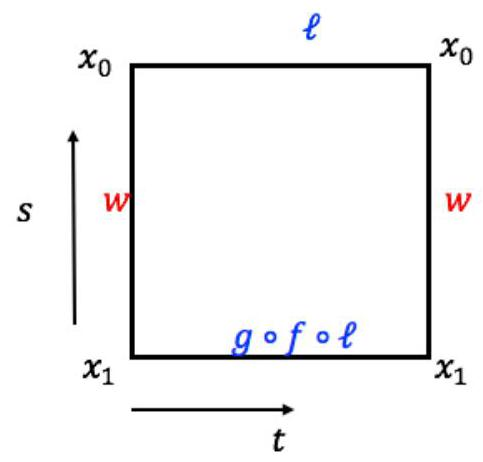
\includegraphics[max width=0.4\textwidth]{images/bo_d2bcsrref24c73avs720_123_558_340_483_462_0.jpg}
\end{center}
\hspace*{3em} 

The homotopy between \(\ell\) and \(g \circ  f \circ  \ell\) motivates us to construct a homotopy between \(\ell\) and \({w}^{-1} \circ  g \circ  f \circ  \ell  \circ  w\) relative to \(\{ 0,1\}\) :

\begin{center}
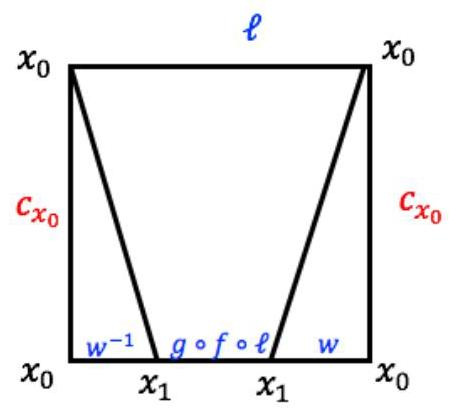
\includegraphics[max width=0.3\textwidth]{images/bo_d2bcsrref24c73avs720_123_631_1071_449_410_0.jpg}
\end{center}
\hspace*{3em} 

Therefore,

\[
\left\lbrack  \ell \right\rbrack   = \left\lbrack  {{w}^{-1}{gf}\ell w}\right\rbrack   = {W}_{\# }\left( \left\lbrack  {{gf}\ell }\right\rbrack  \right)  = \left( {{W}_{\# } \circ  {g}_{ * } \circ  {f}_{ * }}\right) \left\lbrack  \ell \right\rbrack
\]

which follows that \({W}_{\# } \circ  {g}_{ * } \circ  {f}_{ * } = {\operatorname{id}}_{{\pi }_{1}\left( {X,{x}_{0}}\right) }\) . Therfore, \({f}_{ * }\) is injective, \({g}_{ * }\) is surjective.

The similar argument gives

\[
{W}_{\# } \circ  {f}_{ * } \circ  {g}_{ * } = {\operatorname{id}}_{{\pi }_{1}\left( {Y,{y}_{0}}\right) }
\]

Therefore, \({f}_{ * }\) is surjective, \({g}_{ * }\) is injective. The bijectivity is shown.

Definition 12.1 [Simply-Connected] A space \(X\) is simply-connected if \(X\) is path connected, and \(X\) has trivial fundamental group, i.e., \({\pi }_{1}\left( X\right)  = \{ e\}\) for some point \(e \in  X\) .

\begin{itemize}
\item Example 12.4 If \(X\) is contractible, then \(X\) is path-connected. By proposition (12.5), since \(X \simeq  \{ e\}\) , we imply
\end{itemize}

\[
{\pi }_{1}\left( X\right)  \cong  {\pi }_{1}\left( {\{ e\} }\right)  = \{ e\} .
\]

Therefore, all contractible spaces (e.g., \({\mathbb{R}}^{n}\) ) are simply-connected.

However, not all simply-connected spaces are contractible, e.g., \({\pi }_{1}\left( {S}^{2}\right)  \cong  \{ e\}\) , but \({S}^{2}\) is not homotopy equivalent to a point.